%% Início texto

Nesse capítulo iremos apresentar os conceitos fundamentais para entender um ataque de negação de serviço, a aplicação Memcached e seus protocolos. Além disso também será apresentado como efetuar um ataque de reflexão amplificada utilizando o Memcached.

\section{Ataque de negação de serviço}

Um ataque de negação de serviço (\acrfull{DoS}) tem como objetivo principal interromper o acesso de usuários legítimos a serviços ou recursos compartilhados. Esses ataques podem ocorrer em uma variada gama de contextos, de sistemas operacionais a serviços baseados em rede \cite{Peng2007}.

Peng et al.\cite{Peng2007} divide os os ataques DoS em dois tipos. O primeiro compreende os ataques que visam derrubar o sistema da vítima, o segundo tipo inclui os ataques que utilizam um elevado fluxo de tráfego na vítima visando ocupar todos seus recursos. 

Entretanto, Specht et al.\cite{Specht2004} apresenta uma classificação mais detalhada para os ataques DoS. Ele dividi em dois grupos: esgotamento de largura de banda e esgotamento de recurso. A primeira categoria engloba os ataques que visam saturar a largura de banda da vítima com um tráfego não desejado, impedindo assim o tráfego legítimo chegue ao host. Essa categoria é dividida em duas subcategorias: direto e amplificado. A categoria esgotamento de recuso tem o objetivo de esgotar ou encerrar os recursos computacionais da vítima, fazendo com que o host vítima não consiga processar requisições para usuários legítimos. É dividida em duas subcategorias: ataque por exploração de protocolo e vulnerabilidade. Na seção \ref{sec:2.Categoria dos ataques DoS} iremos detalhar melhor essa classificação.

\begin{figure}[H]
     \centering
     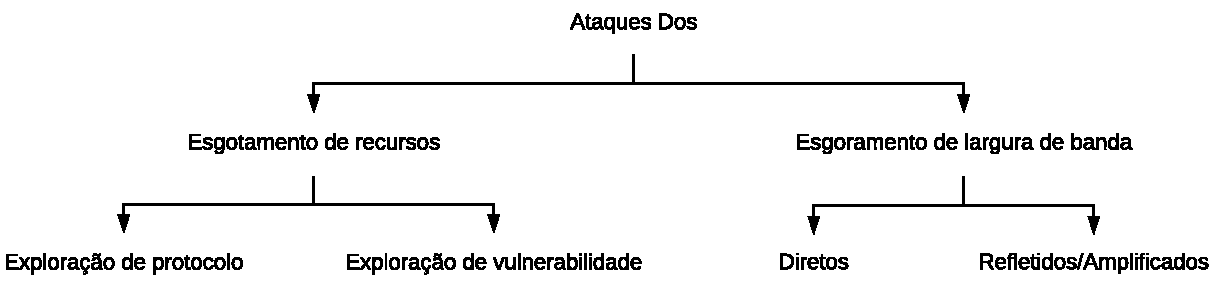
\includegraphics[scale=0.75]{img/ClassificacaoDos.pdf}
     \caption{Classificação dos ataques de negação de serviço}
     \label{img:DDoS}
\end{figure}

\section{Classificação dos ataques DoS} \label{sec:2.Categoria dos ataques DoS}

\subsection{ Esgotamento de recurso }
No ataque de negação de serviço por abuso de protocolo o atacante utiliza uma falha ou característica do protocolo para lançar o ataque. Specht et al.\cite{Specht2004} divide esse tipo de ataque em exploração de protocolo e exploração de vulnerabilidade.

\subsubsection*{ Exploração de protocolo }
Quando o atacante utiliza essa abordagem ele tem como objetivo utilizar uma característica do protocolo para exaurir os recursos do alvo. 

Podemos utilizar como exemplo o ataque TCP SYN \textit{flooding}. Nesse ataque o atacante explora o \textit{three-way handshake} do protocolo TCP, enviando vários pedidos SYN para a vítima com o endereço de IP de origem da vítima. A vítima irá alocar os recursos necessários para estabelecer a conexão TCP, enviará um pacote SYN ACK e irá esperar por um pacote ACK. Como o IP do pacote SYN foi spoofado não teremos a conclusão do \textit{three-way handshake}, fazendo com que o recurso fique alocado por um longo período. Se o atacante conseguir enviar um elevado numero de pacotes TCP SYN, alocando assim um elevado número de conexões, ele pode conseguir exaurir os recursos do alvo efetuando assim o ataque de negação de serviço SYN flooding \cite{tcpsynflood}.

Apesar desse ataque enviar um elevado número pacotes, que é a característica dos ataques de esgoramento de largura de banda, o seu objetivo principal é exaurir os recursos do alvo. Para não causarmos alguma confusão iremos apresentar o ataque \acrfull{RUDY}, que explora o protocolo HTTP. 

O RUDY explora uma fraqueza do protocolo HTTP que foi originalmente desenhado para prover serviços para usuários com um baixo tráfego de rede . Ele utilizado do fato que a operação de HTTP POST permite que a conexão fique aberta por um tempo indeterminado no caso onde os dados chegam a uma taxa muito lenta. O ataque começa com o envio de um pacote legítimo de requisição HTTP POST com campo \textit{content length} possuindo um valor absurdamente grande. Após esse passo inicial o atacante deve começar a injetar pequenos pedaços do dado a uma taxa muito baixa. Isso fará com que o servidor aloque uma grande quantidade de recursos por causa do campo \textit{content length} ser uma valor muito grande por um longo periodo já que os dados chegam a uma taxa muito baixa. Se o atacante conseguir alocar uma grande quantidade de recursos da vítima ele poderá ter um ataque bem sucedido\cite{Alomari2012}.   

\subsubsection*{ Exploração de vulnerabilidade }
Esse tipo de ataque explora uma falha na implementação de um protocolo ou até mesmo o próprio protocolo. Podemos tomar como exemplo uma falha na implementação do protocolo TCP no Windows NT, ao tentar processar um pacote \textit{Out of Band} ocorria um \acrfull{BSoD} \cite{OOB}.

Outro exemplo de ataque que se enquadra nessa categoria é o \textit{Ping of death}. Esse ataque explorava uma falha na implementação do protocolo \acrfull{ICMP} em alguns sistemas, que ao receber um pacote ICMP ECHO maior que 65536 bytes causava um buffer overflow, podendo levar a sua reinicialização\cite{PingofDeath}.

\subsection{ Esgotamento de largura }
Os ataques de negação de serviço volumétricos tem como objetivo saturar a largura de banda da vítima. Podem ser divididos em duas categorias: diretos e refletidos/amplificados \cite{Chang2002}. É indispensável para o atacante utilizar uma arquitetura distribuída para efetuar um ataque bem sucedido nessa categoria de ataque.

\subsubsection*{Ataques diretos}

Esse é que consiste em enviar grande número de pacotes diretamente para vítima com o objetivo de saturar sua largura de banda. Os ataque UDP flood e ICMP flood são exemplos de ataques de negação de serviço dessa subcategoria. Nesses ataques deve-se enviar para a vítima uma grande quantidade de pacotes UDP ou ICMP, tendo como objetivo saturar a largura de banda da vítima. 

\subsubsection*{Ataques refletidos/amplificados}

Uma forma do atacante conseguir mascarar a fonte do ataque é utilizando um
máquina que consiga retransmitir os pacotes do atacante para a vítima. Essa máquina que funciona como mais um agente do ataque é chamada de refletor. 

Possíveis refletores são máquinas na rede que utilizam um protocolo que gere um pacote resposta a partir de um estimulo e que possibilite o spoofing dos pacotes.

Uma máquina com o protocolo TCP pode ser explorada como um refletor, por exemplo. Nesse ataque deve-se enviar pacotes TCP SYN com o endereço spoofado da vítima e os envia para o refletor. O refletor irá responder com pacotes SYN-ACK que serão encaminhados para a vítima. É importante perceber que nesse ataque o refletor será vítima de um ataque TCP SYN \textit{flooding}, então é importante o atacante utilizar vários refletores para não derrubar o refletor e também para não saturar sua largura de banda \cite{Radhakrishnan2011}. 

Um servidor de \acrfull{DNS} mau configurado, deixado em sua configuração padrão, ou um servidor de \acrfull{DNS} público que possui a intenção de disponibilizar seus serviços para a internet são outros exemplos de possíveis refletores. Para se executar o ataque deve-se enviar requisições DNS para o refletor que parecem ser legítimas, entretanto elas estarão spoofadas com o endereço da vítima. Ao receber essa requisição o servidor DNS irá responder para a vítima, já que o pacote recebido possui seu endereço \cite{Anagnostopoulos2013}.

É importante observar que em ambos os casos os refletores podem gerar repostas maiores que as requisições enviadas pelo atacante, causando uma amplificação do ataque pelo refletor. Essa característica do refletor de também se comportar como um amplificador do ataque é excelente no ponto de vista do atacante. Além de possuir um intermediário que irá trazer uma camada a mais de anonimato para a fonte do ataque também irá amplificar seu tráfego gerado, requisitando assim menos de sua infraestruturada para um ataque bem sucedido.

Para medir a eficiência de uma amplificador o cálculo utilizado é dividir o tamanho do pacote de resposta (\textit{response packet}) pelo tamanho do pacote de requisição (\textit{request packet}), esse cálculo nos retorna o fator de amplificação do refletor. Esse fator indica diretamente qual será o impacto de cada refletor no ataque, quanto maior o fator de amplificação melhor é o refletor \cite{Anagnostopoulos2013}.

\begin{equation}
Amplificação = \frac{tamanho(resposta)}{tamanho(pedido)}
\label{cal:Fator_Amp}
\end{equation}

Voltando para o exemplo do servidor DNS, a partir de uma pacote de requisição de 60 bytes podemos conseguir gerar um pacote resposta de até 4000 bytes, gerando uma fator de amplificação de 66 \cite{Anagnostopoulos2013}.

Outro exemplo de refletor com um alto fator de amplificação são servidor Memcached mau configurados expostas a internet. O estudo do Memcached como refletor é o foco do estudo desse trabalho é será abordado na seção \ref{sec:2.Ataque de reflexão amplificado explorando Memcached}.

\section{Ataque de negação de serviço distribuído} \label{sec:2.Ataque de negação de serviço distribuído}

Devido as atuais infraestruturas possuírem uma altas taxa de largura de banda e um grande poder de processamento, ficou inviável para o atacante exaurir os recursos de um determinado alvo com uma única máquina. Para contornar essa barreira os atacantes passaram a utilizar mais fontes de ataque para alcançar um maior poder computacional. 

Essas fontes de ataque geralmente são máquinas comprometidas que passam a ser controladas pelo atacante. Para utilizar essas máquinas como fonte o atacante deve primeiro compromete-las com um \textit{malware} para ter persistência no acesso a máquina comprometida, que passará a ser um bot. Esses bots serão coordenados pelo atacante para lançar o ataque ao mesmo tempo, esse tipo de ataque é chamado de Ataque de Negação de Serviço Distribuído (\acrfull{DDoS}) \cite{Gu2012}. 

\begin{figure}[H]
     \centering
     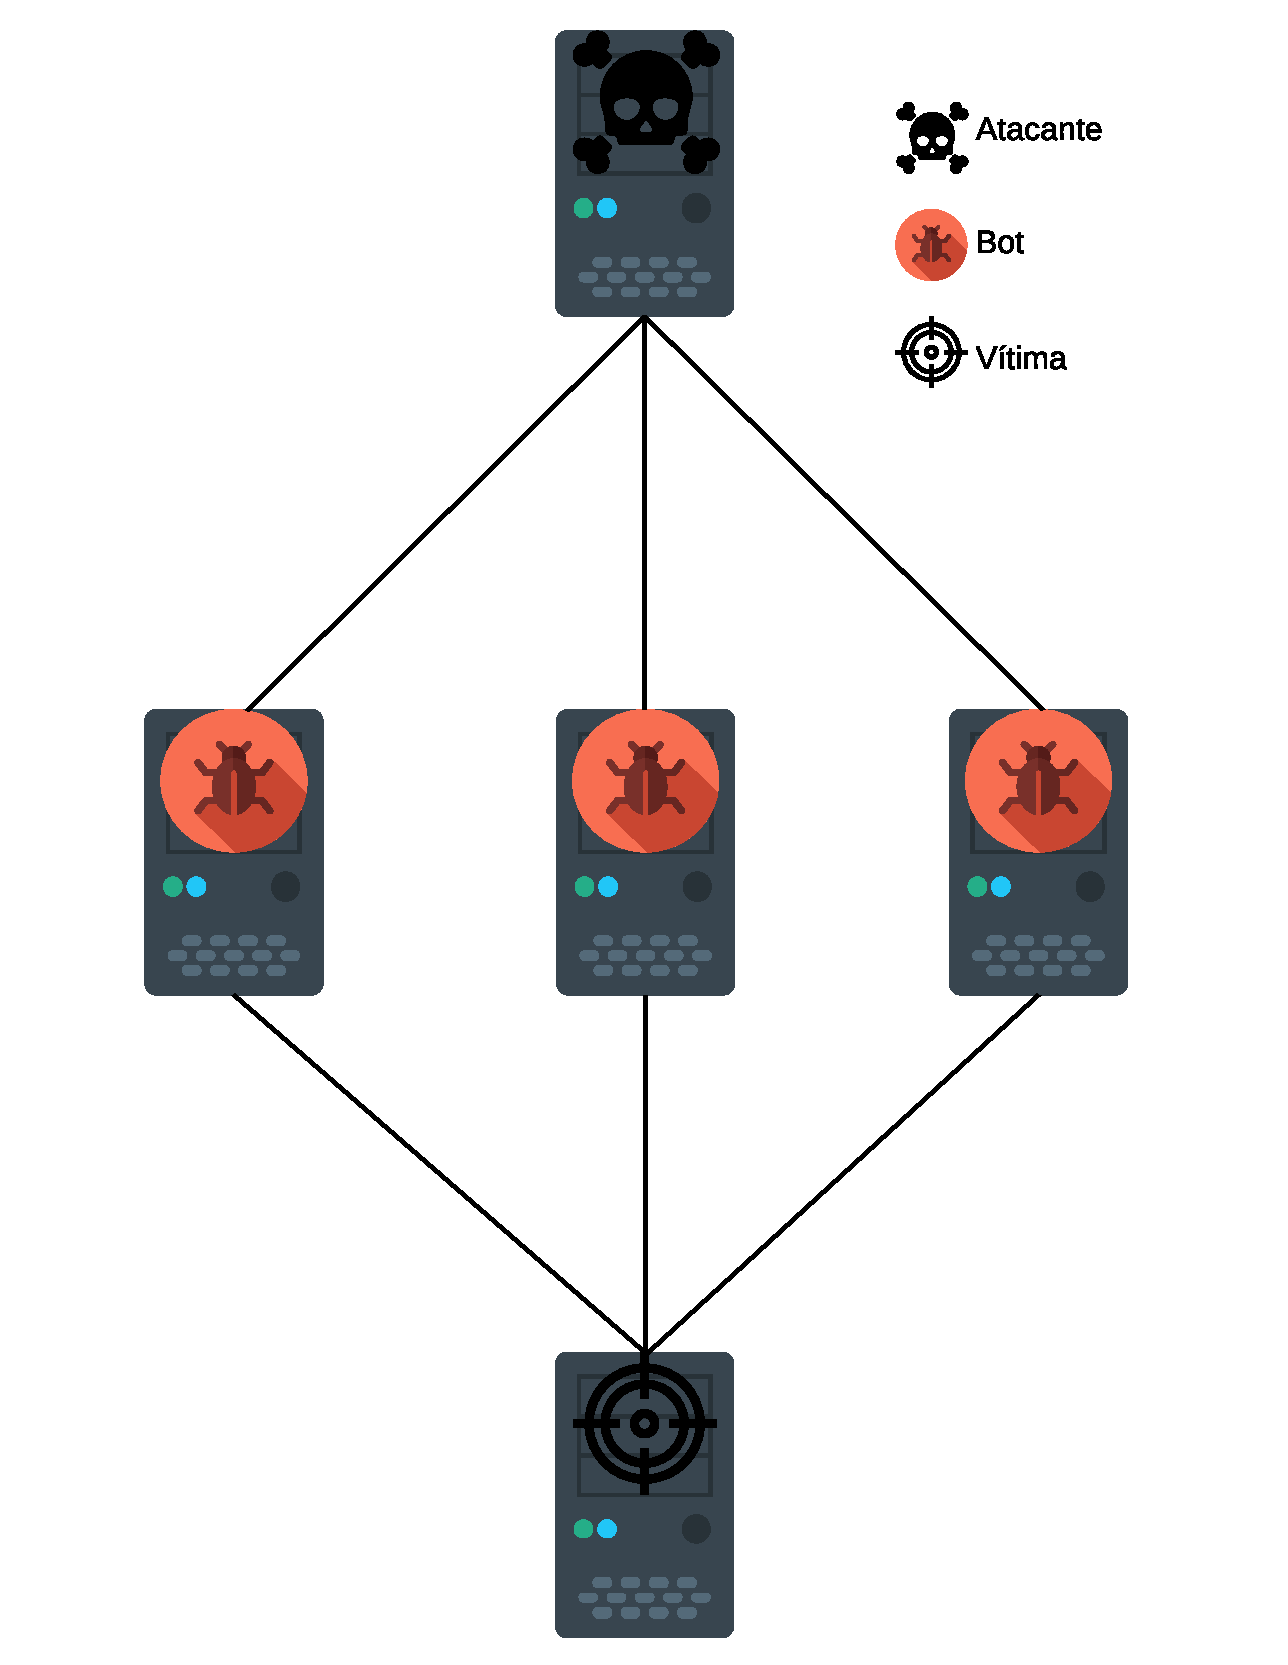
\includegraphics[scale=0.6]{img/DDoS.pdf}
     \caption{Ataque de negação de serviço distribuído}
     \label{img:DDoS}
\end{figure}

Quanto mais bots se tem mais difícil será coordena-los no ataque. Para resolver esse problema algumas arquiteturas surgiram, dando origem às botnets. Alomari etal.\cite{Alomari2012} apresente 3 arquiteturas de Comando e Controle (C\&C) para uma botnet: Agente-Executor, \acrfull{IRC} e Web-based.

Na arquitetura Agente-Executor (Figura \ref{img:DDoS_Architecture_MasterSlave}) os bots são divididos em dois grupos, os agentes que irão fazer o ataque e os executores que são responsáveis por coordenar os agentes. Para iniciar o ataque o atacante necessita apenas enviar os dados necessárias para os executores coordenarem o ataque a uma determinada vítima em uma determinada hora.  
Nessa arquitetura também é possível ter uma rede onde os agentes podem se comunicar com qualquer um dos executores, dando uma maior resiliência à arquitetura.

\begin{figure}[H]
     \centering
     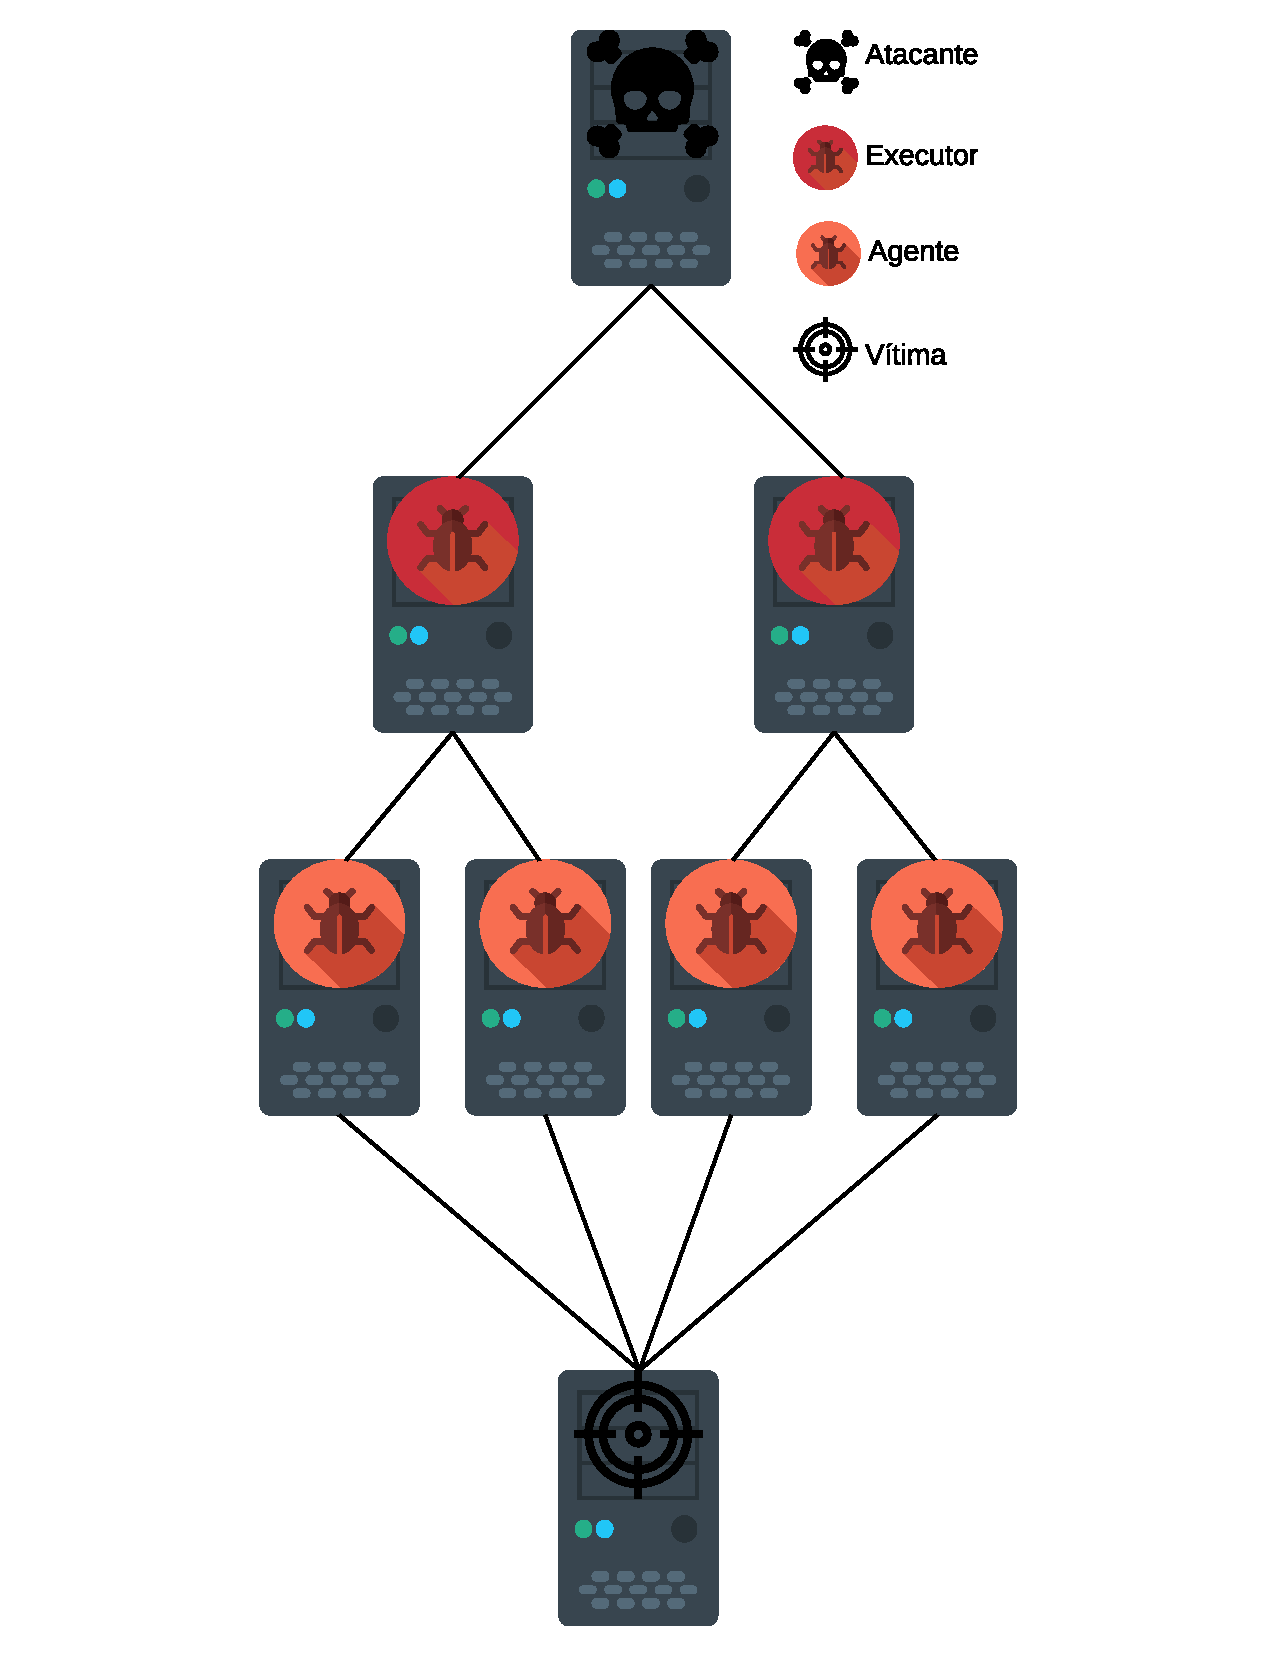
\includegraphics[scale=0.5]{img/DDoS_MS.pdf}
     \caption{Arquitetura Agente-Executor}
     \label{img:DDoS_Architecture_MasterSlave}
\end{figure}

A arquitetura IRC temos um canal IRC como a ligação do atacante aos executores (Figura \ref{img:DDoS_Architecture_IRC}). A vantagem dessa arquitetura em relação a Agente-Executor é que o atacante utiliza um tráfego legítimo, utilizando as portas servidor IRC para iniciar o ataque. Além disso os servidores IRC costumam ter um elevado tráfego, dando um maior anonimato para o atacante. Outra vantagem é que o sistema não precisa armazenar a lista de escravos, já que ele tem esse log no IRC. O atacante pode obter por utilizar vários servidores IRC para uma maior resiliência da botnet.

\begin{figure}[H]
     \centering
     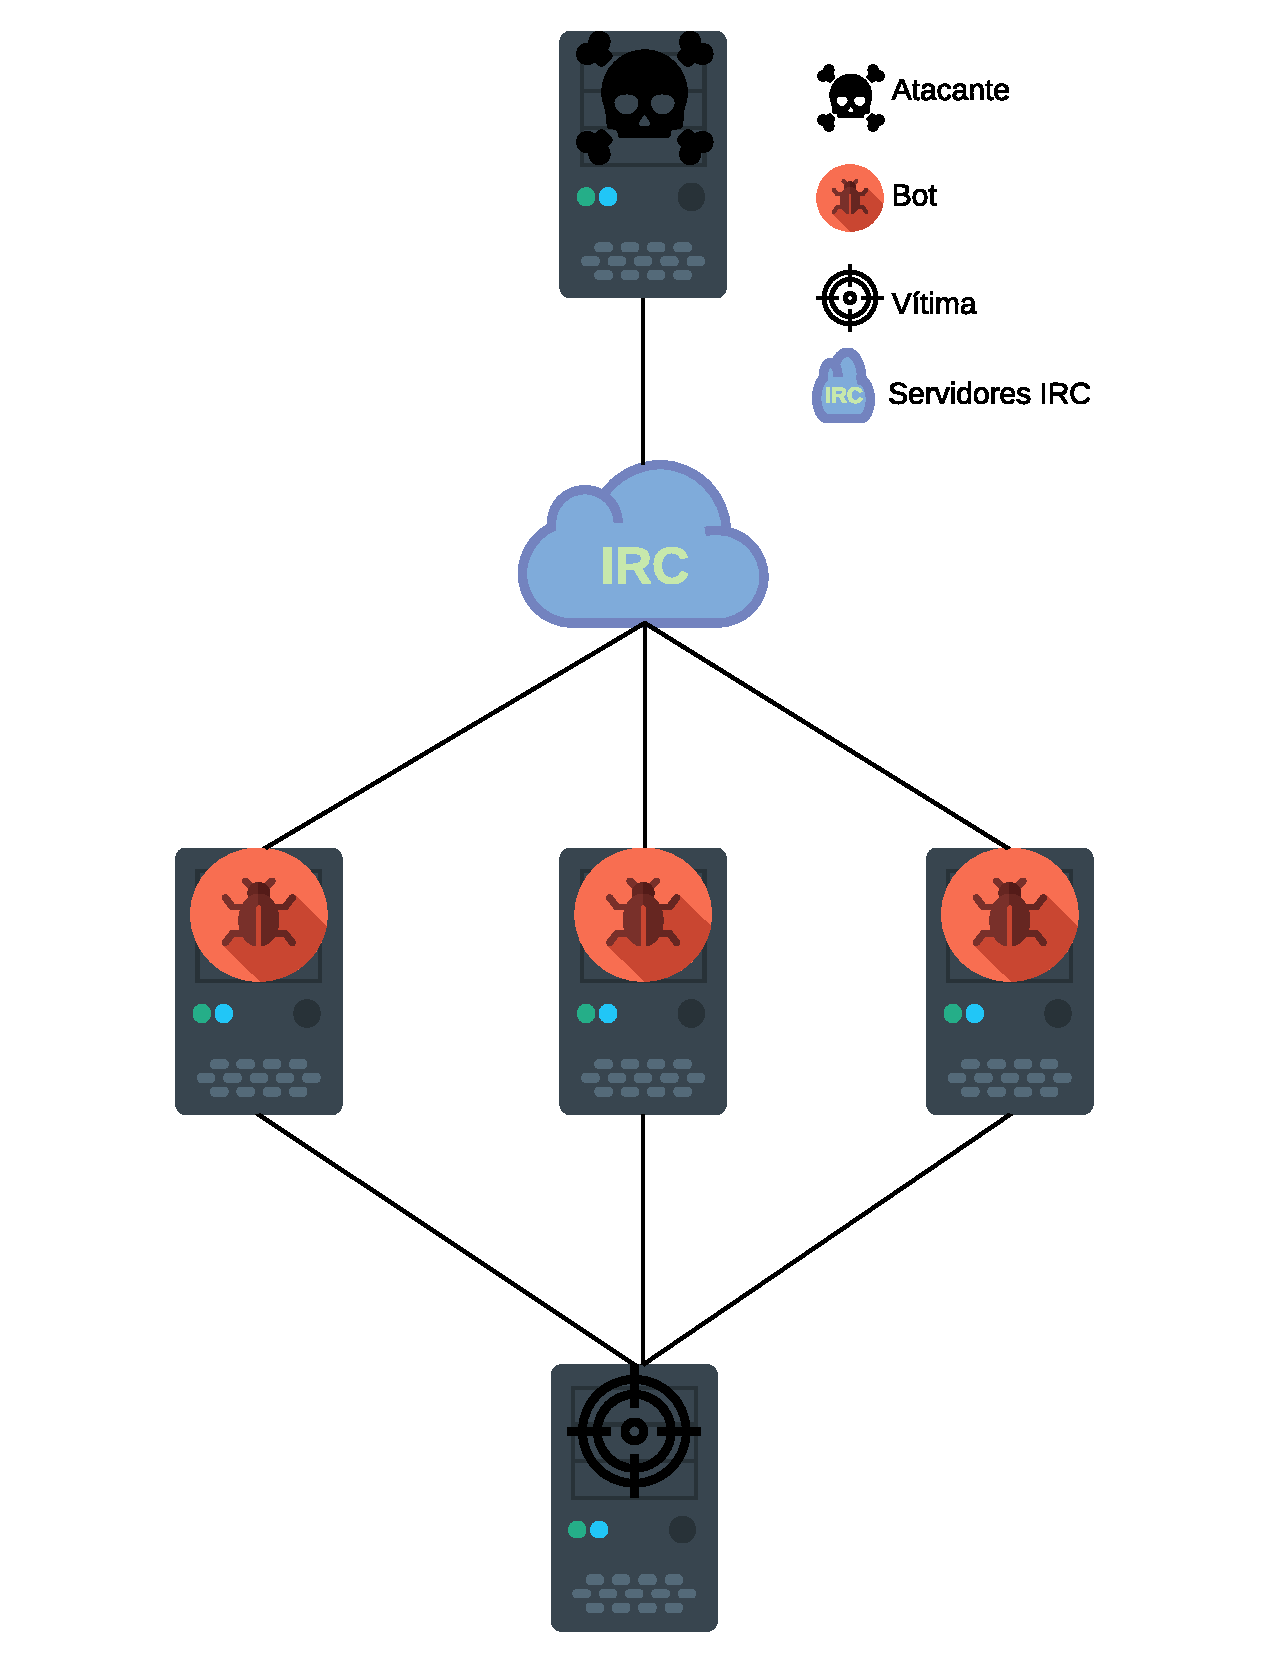
\includegraphics[scale=0.5]{img/DDoS_IRC.pdf}
     \caption{Arquitetura IRC }
     \label{img:DDoS_Architecture_IRC}
\end{figure}

O modelo Web-based e bem parecido com o IRC, a diferença é que ele utilizada uma aplicação web para a comunicação do atacante com os bots. Essa arquitetura possui algumas vantagens em relação a IRC como uma maior flexibilidade para a implementação de scripts mais complexos, o uso do HTTP/HTTPS e um uso mais simplificado.

\section{Ataque de reflexão amplificado explorando Memcached} \label{sec:2.Ataque de reflexão amplificado explorando Memcached}

O Mencached é um sistema distribuído de caching em memória de chave-valor. Sua proposta veio para resolver o problema da dificuldade de escalar um banco de dados devido as garantias para manter as propriedades \acrfull{ACID}. Ele gerencia o caching dos resultados de chamadas de banco de dados, APIs ou qualquer outro dado e é amplamente utilizado para armazenar dados que são frequentemente requisitados, diminuído assim as requisições ao banco de dados.


Exitem dois protocolos que podemos utilizar para a comunicação cliente servidor no Memcached, são eles: protocolo de texto e protocolo binário. A seguir iremos explicar esses dois protocolos focando nos comandos SET/GET e STATS que são os utilizados para efetuar o ataque de reflexão amplificada Memcached.

\subsection{Protocolo de texto}

Nesse protocolo todo comando começa com o nome do comando que se deseja executar, seguido pelos argumentos, se necessário, separados pelo carácter espaço. Todo comando é case-sensitive, em caixa baixa e deve terminar com os caracteres $\backslash$r$\backslash$n \cite{MemcachedTextProtocol}. Os argumentos obrigatórios de uma comando estão entre os caracteres '< >' e os argumentos opcionais estão entre colchetes '[ ]'.

\subsubsection{Armazenado um dado}
Para armazenar um conjunto chave-valor no servidor Memcached utilizaremos o comando `set'. Esse comando possui a seguinte forma:

\begin{lstlisting}
set <key> <flags> <exptime> <bytes> [noreply]\r\n<data block>\r\n
\end{lstlisting}

\begin{itemize}
\item key: a chave que será correspondente ao valor armazenado;
\item flags: Valor de 16 bits que o servidor irá armazenar junto com o dado armazenado que será retornado quando esse dado for requisitado;
\item exptime: tempo que o dado ficará armazenado no servidor. 0 significa que o dado não expira;
\item bytes: número de bytes no campo data block;
\item noreply: parâmetro opcional que instrui o servidor a não enviar um resposta ao cliente;
\item data block: dado que será armazenado no servidor memcached.
\end{itemize}

Caso o noreplay seja omitido no comando set, a resposta do servidor para o cliente será uma das seguintes:

\begin{itemize}
\item STORED$\backslash$r$\backslash$n: indica sucesso;
\item NOT\_STORED$\backslash$r$\backslash$n: dado não foi armazenado.
\end{itemize}

\subsubsection{Requisitando um dado}

Para requisitar um dado do servidor memcached devemos utilizar os comandos 'get' ou 'gets'. Esses comandos possuem a seguinte forma:

\begin{lstlisting}
get <key>\r\n
gets <key>\r\n
\end{lstlisting}


O argumento key corresponde a uma ou mais chaves separadas pelo carácter espaço.


A resposta do servidor segue a seguinte estrutura:

\begin{lstlisting}
VALUE <key> <flags> <bytes> [<cas unique>]\r\n<data block>\r\n
\end{lstlisting}

\begin{itemize}
\item key: a chave armazenada;
\item flags: flag armazenada;
\item bytes: número de bytes no campo data block;
\item cas unique: inteiro de 64 bits que identifica o conjunto chave-valor;
\item data block: dado armazenado no servidor memcached.
\end{itemize}

Caso o servidor não retorne nenhuma resposta significa que o dado não foi armazenado.

\subsubsection{Estatísticas do servidor Memcached}

Para requisitar estatísticas gerais e a configuração do servidor Memcached podemos utilizar o comando stats. Esses comandos possuem a seguinte forma:

\begin{lstlisting}
stats\r\n
\end{lstlisting}

\subsubsection{Utilizando o protocolo UDP}

Ao utilizar o protocolo UDP cada comando possuirá um cabeçalho de 8 bytes. Todo \textit{request} deve conter apenas um datagrama, mas a resposta pode conter um ou mais datagramas.

\begin{figure}[H]
     \centering
     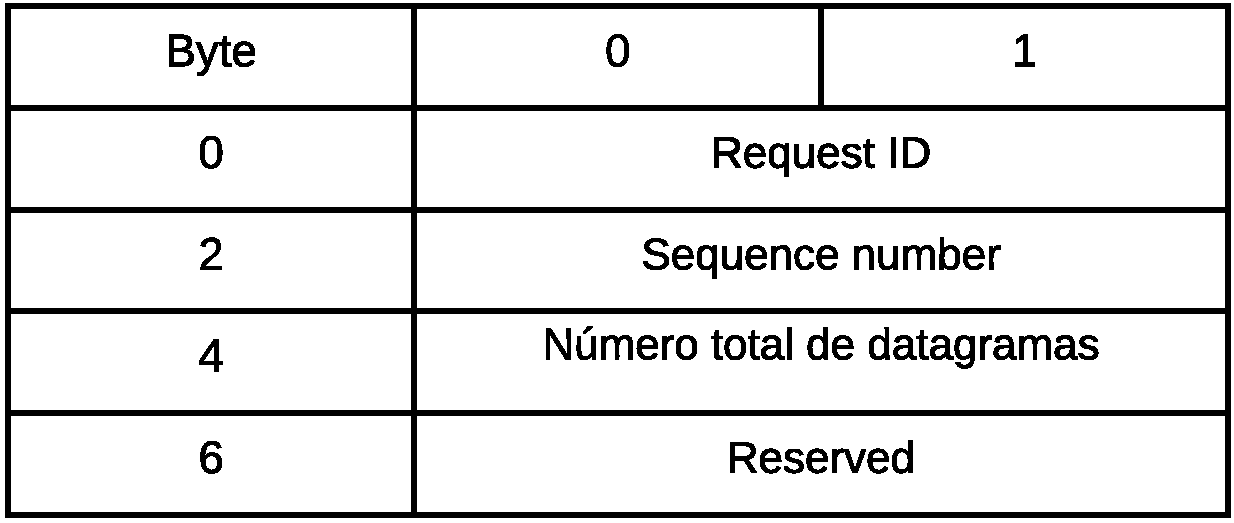
\includegraphics[scale=0.5]{img/CabecalhoTP_UDP.pdf}
     \caption{Cabeçalho UDP protocolo de texto}
     \label{img:UPDtextproto}
\end{figure}

O campo Request ID deve ser fornecido pelo cliente. Normalmente, será um valor crescente monotonicamente a partir de uma semente aleatória, mas o cliente é livre para usar qualquer valor. A resposta do servidor irá conter o mesmo Request ID escolhido pelo cliente. O cliente utiliza esse campo para identificar respostas que possam ser de pedidos pendentes, quaisquer datagrama com um Request ID desconhecido é provavelmente uma resposta atrasada a uma solicitação anterior e deve ser descartada.

O valor do campo Sequence number varia de 0 a n-1, onde n é o número total de datagramas na mensagem. O cliente deve concatenar os payloads dos datagramas para uma dada resposta em ordem numérica de sequencia. A resposta completa terá o mesmo formato de uma resposta enviado com o protocolo TCP(incluindo terminação $\backslash$r$\backslash$n sequências).

O campo Reserved é reservado para uso futuro e deve ter o valor 0.

\subsection{Protocolo binário}

Os pacotes binários Memcached possuem um campo obrigatório que é o cabeçalho e mais três campos que são opcionais , são eles Command-specific extras, Key, e Value. Como apresentado na Figura \ref{img:Estrtutura pkg_Mem}. \cite{MemcachedBinaryProtocol}

\begin{figure}[H]
     \centering
     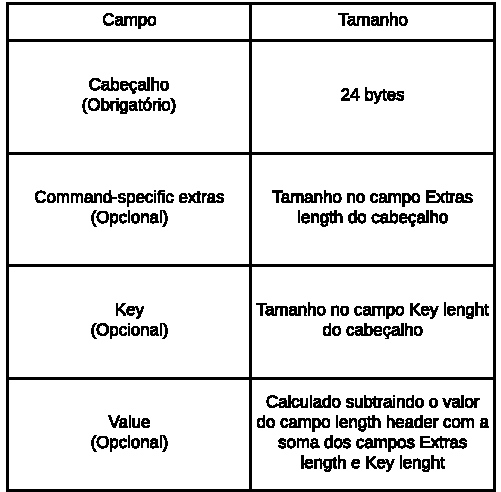
\includegraphics[scale=1]{img/Estrutura_pacote_Memcached.pdf}
     \caption{Estrutura geral do pacote Memcached }
     \label{img:Estrtutura pkg_Mem}
\end{figure}

Os comandos possuem dois tipos de cabeçalho para os pacotes, um para o requisições (pacote \textit{request}) Figura \ref{img:Estrtutura request}, e outro para respostas (pacote \textit{response}) Figura \ref{img:Estrtutura response}. Os dois possuem 9 campos com a única diferença entre eles é a existência do campo bvucket id ou Status. 

\begin{figure}[H]
     \centering
     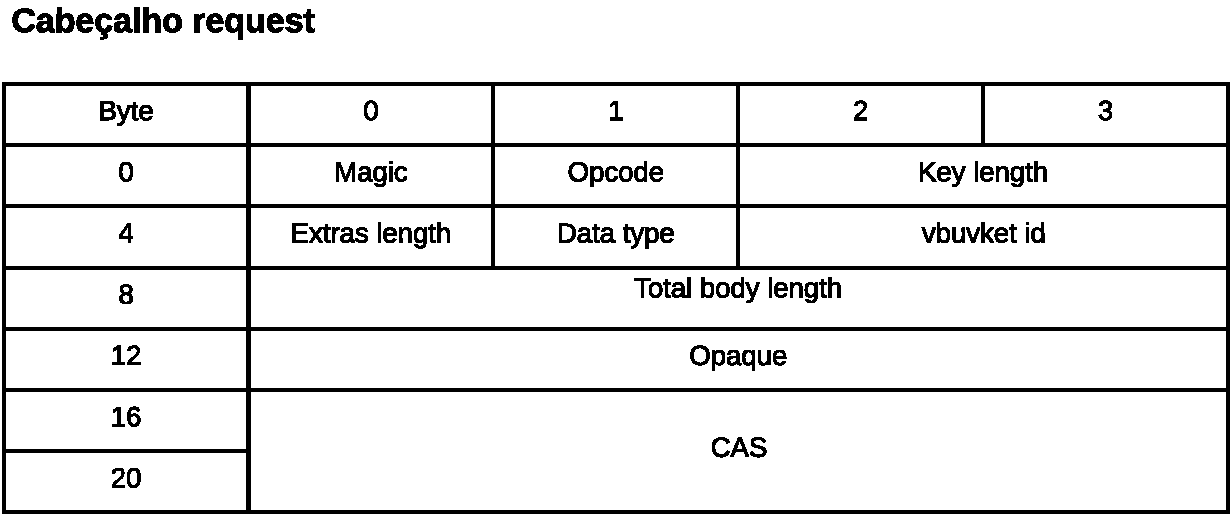
\includegraphics[scale=0.6]{img/Memcached_request_header.pdf}
     \caption{Estrutura do pacote \textit{request} Memcached }
     \label{img:Estrtutura request}
\end{figure}

\begin{figure}[H]
     \centering
     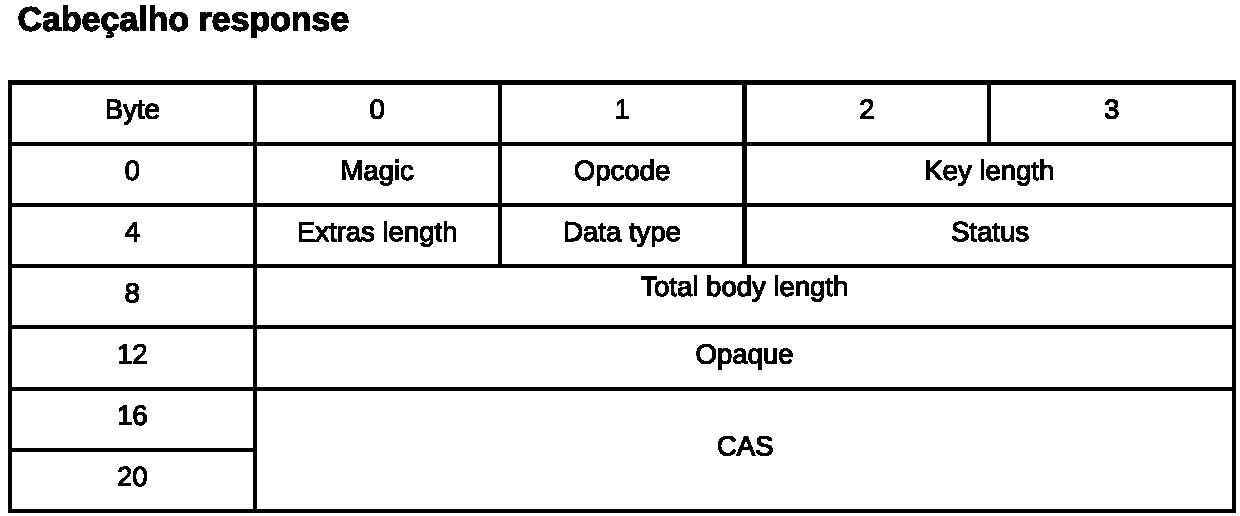
\includegraphics[scale=0.6]{img/Memcached_response_header.pdf}
     \caption{Estrutura do pacote \textit{response} Memcached }
     \label{img:Estrtutura response}
\end{figure}

\begin{itemize}
\item Magic: identificação da versão do protocolo. Para cada versão do protocolo é usado um valor para os pacote request o outro para o response;
\item Opcode: identificação do comando a ser executado (Figura \ref{img:Opcode});
\item Key length: tamanho em bytes do campo Key;
\item Extras length: tamanho em bytes do campo Command-specific extras; 
\item Data type: reservado para uso futuro.
\item vbucket id: o bucket virtual para o comando;
\item Status: status da resposta, diferente de zero se ocorrer um erro (Figura \ref{img:Status_Code});
\item Total body length: tamanho em bytes da soma dos tamanhos dos campos Extras, Key e Value;
\item Opaque: Dado que será copiado de volta na resposta;
\item CAS: Data version check.
\end{itemize}

Na Figura \ref{img:Opcode} apresentamos os Opcodes dos comandos Get, Set e Stat. O comando Get busca por uma chave e retorna o valor, possui campo opcional Key para o \textit{request} e para o \textit{response} possui Key e Value. O comando Set armazena uma dado (chave-valor) no servidor, possui campo opcional . E o comando Stat retorna os dados de status do servidor.

\begin{figure}[H]
     \centering
     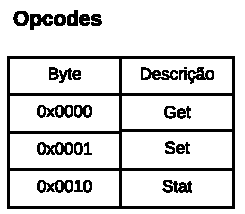
\includegraphics[scale=1]{img/Opcode_Memcached.pdf}
     \caption{Códigos campo Opcode (apenas os utilizados no ataque) }
     \label{img:Opcode}
\end{figure}

\begin{figure}[H]
     \centering
     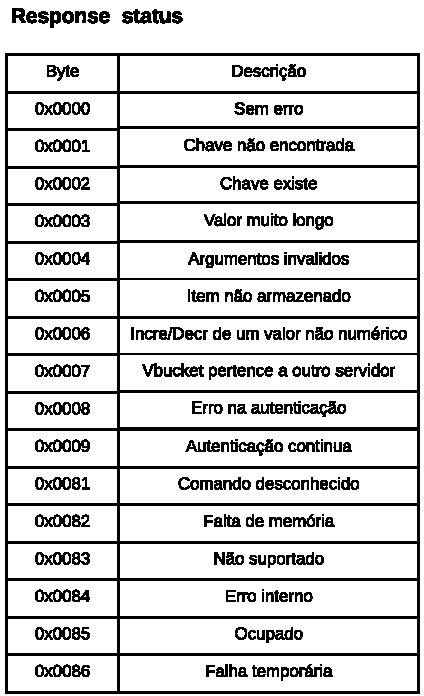
\includegraphics[scale=1]{img/Response_Status.pdf}
     \caption{Códigos do campo Status }
     \label{img:Status_Code}
\end{figure}

Todo comunicação é iniciada por um pacote de \textit{request} enviado pelo cliente, e o servidor irá responder com 0 ou múltiplos pacotes para cada pedido.  Se o campo Status de um pacote \textit{response} é diferente de 0, o corpo do pacote irá conter a mensagem de erro. Se for zero o campo Opcode irá definir o layout da estrutura do pacote.

\subsubsection*{Efetuando o ataque}

O Memcached não possui controle de acesso, não sendo desenhado para operar com suas portas expostas para a internet. Porém, algumas empresas vem utilizando o Memcached com suas portas abertas para a internet sem os devidos cuidados básicos para evitar o uso de seus servidores como refletores.

Para ser possível utilizar um servidor Memcached como refletor/amplificador é necessário que o servidor Memcached tenha o protocolo UDP habilitado e exposto a internet para qualquer endereço da rede. 

Existem duas formas de explorar o servidor como refletor/amplificador. A primeira, e mais simples, é forjar um pacote Stat \textit{request} Memcached com o endereço da vítima no campo de endereço da fonte do pacote IP. O servidor irá responder para a vítima com um pacote Stat \textit{response}.

O segundo método exige um certo preparo do servidor antes de iniciar o ataque. O atacante deve saber qual o valor máximo permitido para os valores armazenados. Para obter esse dado o atacante deve utilizar pacotes Stat para encontrar um tamanho máximo que podemos armazenar no valor. Após escolher os melhores refletores, o atacante deve armazenar os dados de chave-valor em cada refletor, respeitando os limites encontrados no passo anterior para ter certeza que o dado foi armazenado. Como o dado de chave-valor armazenado o ataque pode começar, para isso o atacante deve enviar pacotes Get \textit{request} forjados com o endereço IP da vítima, isso implicará que o servidor Memcached irá responder com um pacote Get \textit{response} para a vítima.

\begin{figure}[H]
     \centering
     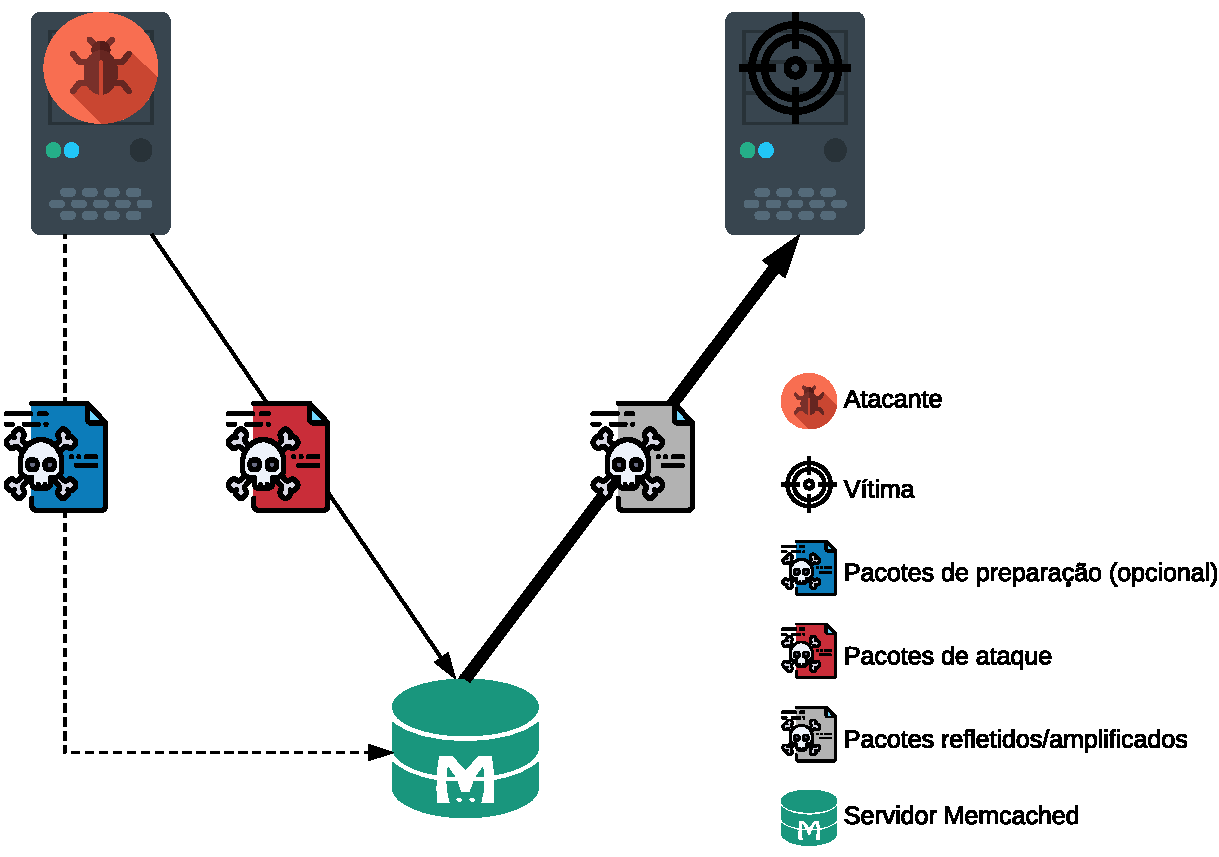
\includegraphics[scale=0.6]{img/DDoS_Memcached.pdf}
     \caption{Uso do refletor Memcached}
     \label{img:Status_Code}
\end{figure}

Para calcular a eficiência do ataque iremos utilizar a razão do tamanho do pacote de resposta pelo de requisição, como apresentado na equação \ref{cal:AmpFactor}. Essa valor nos dará a amplificação do ataque e quanto maior for essa valor mais eficiente é o ataque. Iremos considerar nos cálculos os cabeçalhos IP e UDP já que eles fazem parte do pacote que será enviado na rede e existiu um esforço computacional para gerá-los.

\begin{equation}
Amplificação = \frac{Resposta}{Requisição}
\label{cal:AmpFactor}
\end{equation}

Para calcular o fator de amplificação do método GET/SET iremos considerar a fase do uso do pacote SET como uma preparação, o cálculo do fator de amplificação utilizará apenas os pacotes GET. Assim temos a equação \ref{cal:Fator_Memcached2} como o fator de amplificação do segundo método.

\begin{equation}
Amplificação = \frac{Ip + Udp + Header + Key + Value}{Ip + Udp + Header + Payload} = 1 + \frac{Value}{Ip + Udp +Header + Payload}
\label{cal:Fator_Memcached2}
\end{equation}

O ataque de negação de serviço utilizando Memcached tem um grande potencial para disponibilizar uma alta amplificação. No capítulo \ref{sec:Apresetacao} iremos apresentar os testes e análise do uso de um servidor Memcached em um ataque DoS.